\documentclass{beamer}
\beamertemplatenavigationsymbolsempty
\usecolortheme{beaver}
\setbeamertemplate{blocks}[rounded=true, shadow=true]
\setbeamertemplate{footline}[page number]
%
\usepackage[utf8]{inputenc}
\usepackage[english,russian]{babel}
\usepackage{amssymb,amsfonts,amsmath,mathtext}
\usepackage{subfig}
\usepackage[all]{xy} % xy package for diagrams
\usepackage{array}
\usepackage{multicol}% many columns in slide
\usepackage{hyperref}% urls
\usepackage{hhline}%tables
% Your figures are here:
\graphicspath{ {fig/} {../figures/} }

%----------------------------------------------------------------------------------------------------------
\title[\hbox to 56mm{Ускоренные безградиентные методы}]{Ускоренные методы нулевого порядка в гладкой выпуклой стохастической оптимизации}
\author[Ф.\,А. Хафизов]{Фанис Адикович Хафизов}
\institute{Московский физико-технический институт}
\date{\footnotesize
\par\smallskip\emph{Курс:} Автоматизация научных исследований\par (практика, В.\,В.~Стрижов)/Группа 105
\par\smallskip\emph{Эксперт:} А.\,Н.~Безносиков
\par\smallskip\emph{Консультант:} А.\,И.~Богданов
\par\bigskip\small 2024}
%----------------------------------------------------------------------------------------------------------
\begin{document}
%----------------------------------------------------------------------------------------------------------
\begin{frame}
\thispagestyle{empty}
\maketitle
\end{frame}
%-----------------------------------------------------------------------------------------------------
% \begin{frame}{Цель исследования}
%\begin{block}{Решается задача}
%\end{block}
% \end{frame}
%-----------------------------------------------------------------------------------------------------
\begin{frame}{Доклад с одним слайдом}

\begin{columns}[c]
\column{0.5\textwidth}
\begin{figure}
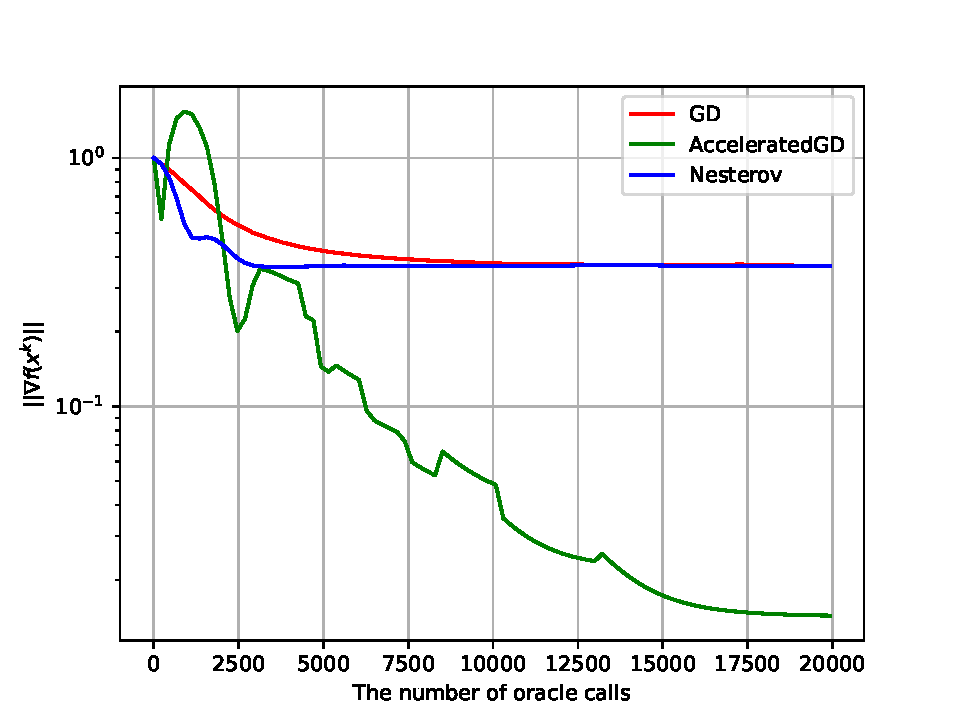
\includegraphics[width=1.0\textwidth]{Non_stochastic_Logreg_GD_AGD_Nesterov_15_1e-07_1e-05.pdf}
    \caption{Зависимость $\|\nabla f(x^k)\|$ от числа итераций, задача логистической регрессии}
\end{figure}
\column{0.5\textwidth}
\begin{figure}
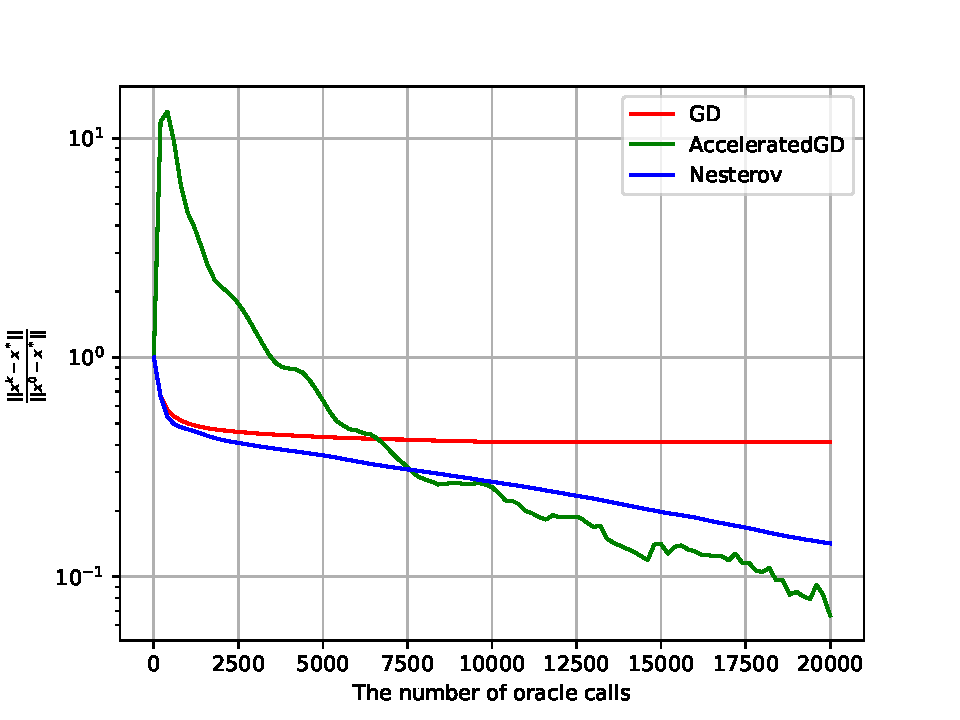
\includegraphics[width=1.0\textwidth]{Deterministic_quadratic_GD_AGD_Nesterov_15.pdf}
    \caption{Зависимость $\frac{\|x^k - x^*\|}{\|x^0 - x^*\|}$ от числа итераций, квадратичная задача минимизации}
    \end{figure}
\end{columns}

\end{frame}


%----------------------------------------------------------------------------------------------------------
% \begin{frame}{Постановка задачи}
%
% \end{frame}
%----------------------------------------------------------------------------------------------------------
% \begin{frame}{Решение}
% \begin{columns}[c]
% \column{0.6\textwidth}
%     Столбец 1
% \column{0.4\textwidth}
%     Столбец 2
% \end{columns}
% \end{frame}
%----------------------------------------------------------------------------------------------------------
% \begin{frame}{Вычислительный эксперимент}
%
%  Что зритель видит на графике.
%
% \includegraphics[width=0.8\textwidth]{ErrorFunction}
%
% О чем говорит этот график.
%
% \end{frame}
%----------------------------------------------------------------------------------------------------------
% \begin{frame}{Заключение}
%     \begin{block}{Перечислите ваши результаты}
%     \begin{itemize}
%         \item предложен метод,
%         \item доказана теорема.
%     \end{itemize}
%     \end{block}
% \end{frame}
%----------------------------------------------------------------------------------------------------------

\end{document} 
